\documentclass[twoside]{book}

% Packages required by doxygen
\usepackage{fixltx2e}
\usepackage{calc}
\usepackage{doxygen}
\usepackage[export]{adjustbox} % also loads graphicx
\usepackage{graphicx}
\usepackage[utf8]{inputenc}
\usepackage{makeidx}
\usepackage{multicol}
\usepackage{multirow}
\PassOptionsToPackage{warn}{textcomp}
\usepackage{textcomp}
\usepackage[nointegrals]{wasysym}
\usepackage[table]{xcolor}

% Font selection
\usepackage[T1]{fontenc}
\usepackage[scaled=.90]{helvet}
\usepackage{courier}
\usepackage{amssymb}
\usepackage{sectsty}
\renewcommand{\familydefault}{\sfdefault}
\allsectionsfont{%
  \fontseries{bc}\selectfont%
  \color{darkgray}%
}
\renewcommand{\DoxyLabelFont}{%
  \fontseries{bc}\selectfont%
  \color{darkgray}%
}
\newcommand{\+}{\discretionary{\mbox{\scriptsize$\hookleftarrow$}}{}{}}

% Page & text layout
\usepackage{geometry}
\geometry{%
  a4paper,%
  top=2.5cm,%
  bottom=2.5cm,%
  left=2.5cm,%
  right=2.5cm%
}
\tolerance=750
\hfuzz=15pt
\hbadness=750
\setlength{\emergencystretch}{15pt}
\setlength{\parindent}{0cm}
\setlength{\parskip}{3ex plus 2ex minus 2ex}
\makeatletter
\renewcommand{\paragraph}{%
  \@startsection{paragraph}{4}{0ex}{-1.0ex}{1.0ex}{%
    \normalfont\normalsize\bfseries\SS@parafont%
  }%
}
\renewcommand{\subparagraph}{%
  \@startsection{subparagraph}{5}{0ex}{-1.0ex}{1.0ex}{%
    \normalfont\normalsize\bfseries\SS@subparafont%
  }%
}
\makeatother

% Headers & footers
\usepackage{fancyhdr}
\pagestyle{fancyplain}
\fancyhead[LE]{\fancyplain{}{\bfseries\thepage}}
\fancyhead[CE]{\fancyplain{}{}}
\fancyhead[RE]{\fancyplain{}{\bfseries\leftmark}}
\fancyhead[LO]{\fancyplain{}{\bfseries\rightmark}}
\fancyhead[CO]{\fancyplain{}{}}
\fancyhead[RO]{\fancyplain{}{\bfseries\thepage}}
\fancyfoot[LE]{\fancyplain{}{}}
\fancyfoot[CE]{\fancyplain{}{}}
\fancyfoot[RE]{\fancyplain{}{\bfseries\scriptsize Generated by Doxygen }}
\fancyfoot[LO]{\fancyplain{}{\bfseries\scriptsize Generated by Doxygen }}
\fancyfoot[CO]{\fancyplain{}{}}
\fancyfoot[RO]{\fancyplain{}{}}
\renewcommand{\footrulewidth}{0.4pt}
\renewcommand{\chaptermark}[1]{%
  \markboth{#1}{}%
}
\renewcommand{\sectionmark}[1]{%
  \markright{\thesection\ #1}%
}

% Indices & bibliography
\usepackage{natbib}
\usepackage[titles]{tocloft}
\setcounter{tocdepth}{3}
\setcounter{secnumdepth}{5}
\makeindex

% Hyperlinks (required, but should be loaded last)
\usepackage{ifpdf}
\ifpdf
  \usepackage[pdftex,pagebackref=true]{hyperref}
\else
  \usepackage[ps2pdf,pagebackref=true]{hyperref}
\fi
\hypersetup{%
  colorlinks=true,%
  linkcolor=blue,%
  citecolor=blue,%
  unicode%
}

% Custom commands
\newcommand{\clearemptydoublepage}{%
  \newpage{\pagestyle{empty}\cleardoublepage}%
}

\usepackage{caption}
\captionsetup{labelsep=space,justification=centering,font={bf},singlelinecheck=off,skip=4pt,position=top}

%===== C O N T E N T S =====

\begin{document}

% Titlepage & ToC
\hypersetup{pageanchor=false,
             bookmarksnumbered=true,
             pdfencoding=unicode
            }
\pagenumbering{alph}
\begin{titlepage}
\vspace*{7cm}
\begin{center}%
{\Large My Project }\\
\vspace*{1cm}
{\large Generated by Doxygen 1.8.14}\\
\end{center}
\end{titlepage}
\clearemptydoublepage
\pagenumbering{roman}
\tableofcontents
\clearemptydoublepage
\pagenumbering{arabic}
\hypersetup{pageanchor=true}

%--- Begin generated contents ---
\chapter{Hierarchical Index}
\section{Class Hierarchy}
This inheritance list is sorted roughly, but not completely, alphabetically\+:\begin{DoxyCompactList}
\item \contentsline{section}{Customer\+Order}{\pageref{class_customer_order}}{}
\item \contentsline{section}{Item}{\pageref{class_item}}{}
\begin{DoxyCompactList}
\item \contentsline{section}{Task}{\pageref{class_task}}{}
\end{DoxyCompactList}
\item \contentsline{section}{Item\+Info}{\pageref{struct_item_info}}{}
\item \contentsline{section}{Line\+Manager}{\pageref{class_line_manager}}{}
\item \contentsline{section}{Utilities}{\pageref{class_utilities}}{}
\end{DoxyCompactList}

\chapter{Class Index}
\subsection{Class List}
Here are the classes, structs, unions and interfaces with brief descriptions\+:\begin{DoxyCompactList}
\item\contentsline{section}{\hyperlink{struct_coord_struct}{Coord\+Struct} }{\pageref{struct_coord_struct}}{}
\end{DoxyCompactList}

\chapter{Class Documentation}
\hypertarget{class_customer_order}{}\section{Customer\+Order Class Reference}
\label{class_customer_order}\index{Customer\+Order@{Customer\+Order}}
\subsection*{Public Member Functions}
\begin{DoxyCompactItemize}
\item 
\mbox{\Hypertarget{class_customer_order_a00e1cb818605bcd7457febba4ca9e166}\label{class_customer_order_a00e1cb818605bcd7457febba4ca9e166}} 
{\bfseries Customer\+Order} (std\+::string \&)
\item 
\mbox{\Hypertarget{class_customer_order_a88603e0493f6bf116b6301be6f36b152}\label{class_customer_order_a88603e0493f6bf116b6301be6f36b152}} 
{\bfseries Customer\+Order} (\mbox{\hyperlink{class_customer_order}{Customer\+Order}} \&)
\item 
\mbox{\Hypertarget{class_customer_order_a1a83b197a0ca27da950b7321273c46a5}\label{class_customer_order_a1a83b197a0ca27da950b7321273c46a5}} 
\mbox{\hyperlink{class_customer_order}{Customer\+Order}} \& {\bfseries operator=} (\mbox{\hyperlink{class_customer_order}{Customer\+Order}} \&)=delete
\item 
\mbox{\Hypertarget{class_customer_order_ac46e4af986aecae685a6d745d98b0381}\label{class_customer_order_ac46e4af986aecae685a6d745d98b0381}} 
{\bfseries Customer\+Order} (\mbox{\hyperlink{class_customer_order}{Customer\+Order}} \&\&)
\item 
\mbox{\Hypertarget{class_customer_order_a0567505c22f226c50eeb925e611b411b}\label{class_customer_order_a0567505c22f226c50eeb925e611b411b}} 
\mbox{\hyperlink{class_customer_order}{Customer\+Order}} \& {\bfseries operator=} (\mbox{\hyperlink{class_customer_order}{Customer\+Order}} \&\&)
\item 
\mbox{\Hypertarget{class_customer_order_a36aede6a3339abdd2f476119dea55cf4}\label{class_customer_order_a36aede6a3339abdd2f476119dea55cf4}} 
bool {\bfseries get\+Order\+Fill\+State} ()
\item 
\mbox{\Hypertarget{class_customer_order_a108f3b4e8ebe8075642b24a5d06ed869}\label{class_customer_order_a108f3b4e8ebe8075642b24a5d06ed869}} 
bool {\bfseries get\+Item\+Fill\+State} (std\+::string)
\item 
\mbox{\Hypertarget{class_customer_order_a935ba17e7f591b90bde0c3dc5b5eb8e5}\label{class_customer_order_a935ba17e7f591b90bde0c3dc5b5eb8e5}} 
void {\bfseries fill\+Item} (\mbox{\hyperlink{class_item}{Item}} \&, std\+::ostream \&)
\item 
\mbox{\Hypertarget{class_customer_order_a7ae264df8502dca90853887064922abe}\label{class_customer_order_a7ae264df8502dca90853887064922abe}} 
void {\bfseries Display} (std\+::ostream \&)
\end{DoxyCompactItemize}


The documentation for this class was generated from the following file\+:\begin{DoxyCompactItemize}
\item 
Customer\+Order.\+h\end{DoxyCompactItemize}

\hypertarget{class_item}{}\section{Item Class Reference}
\label{class_item}\index{Item@{Item}}
Inheritance diagram for Item\+:\begin{figure}[H]
\begin{center}
\leavevmode
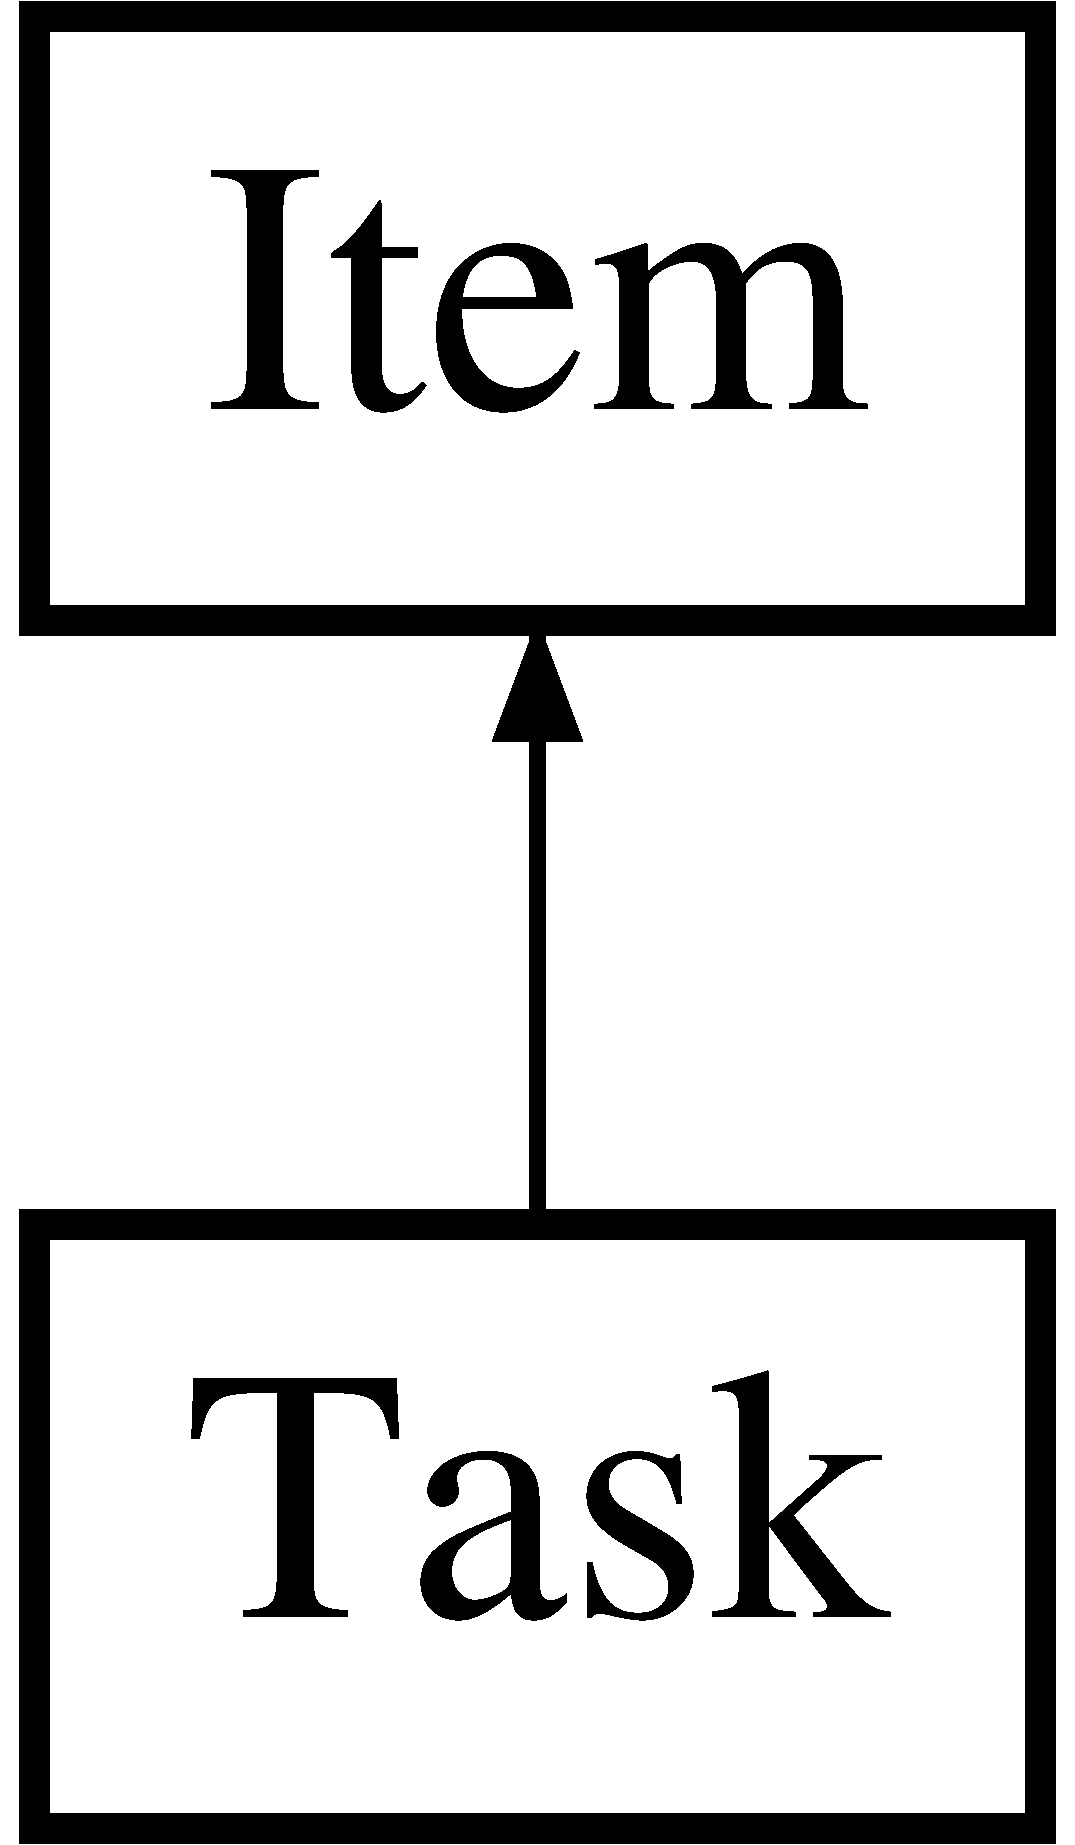
\includegraphics[height=2.000000cm]{class_item}
\end{center}
\end{figure}
\subsection*{Public Member Functions}
\begin{DoxyCompactItemize}
\item 
\mbox{\hyperlink{class_item_ab7cd3059adc4e1639714eea98d0dafc6}{Item}} (const std\+::string \&record)
\item 
const std\+::string \& \mbox{\hyperlink{class_item_a906722df9ab3f424d32c4106ff64aa15}{get\+Name}} () const
\item 
const unsigned int \mbox{\hyperlink{class_item_a73bb3db4f7f0c571d6527d70875db284}{get\+Serial\+Number}} () const
\item 
const unsigned int \mbox{\hyperlink{class_item_ad4d1e93eb012fb0124fa274284fb415c}{get\+Quantity}} () const
\item 
void \mbox{\hyperlink{class_item_ae54aa11885082b7f5e37a925dace0c65}{update\+Quantity}} ()
\item 
void \mbox{\hyperlink{class_item_a41852668dc58d933f786007835dbd8b5}{display}} (std\+::ostream \&, bool) const
\end{DoxyCompactItemize}


\subsection{Constructor \& Destructor Documentation}
\mbox{\Hypertarget{class_item_ab7cd3059adc4e1639714eea98d0dafc6}\label{class_item_ab7cd3059adc4e1639714eea98d0dafc6}} 
\index{Item@{Item}!Item@{Item}}
\index{Item@{Item}!Item@{Item}}
\subsubsection{\texorpdfstring{Item()}{Item()}}
{\footnotesize\ttfamily Item\+::\+Item (\begin{DoxyParamCaption}\item[{const std\+::string \&}]{record }\end{DoxyParamCaption})}

custom constructor parses data from string !$>$ 

\subsection{Member Function Documentation}
\mbox{\Hypertarget{class_item_a41852668dc58d933f786007835dbd8b5}\label{class_item_a41852668dc58d933f786007835dbd8b5}} 
\index{Item@{Item}!display@{display}}
\index{display@{display}!Item@{Item}}
\subsubsection{\texorpdfstring{display()}{display()}}
{\footnotesize\ttfamily void Item\+::display (\begin{DoxyParamCaption}\item[{std\+::ostream \&}]{os,  }\item[{bool}]{full }\end{DoxyParamCaption}) const}

display function !$>$ \mbox{\Hypertarget{class_item_a906722df9ab3f424d32c4106ff64aa15}\label{class_item_a906722df9ab3f424d32c4106ff64aa15}} 
\index{Item@{Item}!get\+Name@{get\+Name}}
\index{get\+Name@{get\+Name}!Item@{Item}}
\subsubsection{\texorpdfstring{get\+Name()}{getName()}}
{\footnotesize\ttfamily const std\+::string \& Item\+::get\+Name (\begin{DoxyParamCaption}{ }\end{DoxyParamCaption}) const}

function return product name !$>$ \mbox{\Hypertarget{class_item_ad4d1e93eb012fb0124fa274284fb415c}\label{class_item_ad4d1e93eb012fb0124fa274284fb415c}} 
\index{Item@{Item}!get\+Quantity@{get\+Quantity}}
\index{get\+Quantity@{get\+Quantity}!Item@{Item}}
\subsubsection{\texorpdfstring{get\+Quantity()}{getQuantity()}}
{\footnotesize\ttfamily const unsigned int Item\+::get\+Quantity (\begin{DoxyParamCaption}{ }\end{DoxyParamCaption}) const}

function return product quantity !$>$ \mbox{\Hypertarget{class_item_a73bb3db4f7f0c571d6527d70875db284}\label{class_item_a73bb3db4f7f0c571d6527d70875db284}} 
\index{Item@{Item}!get\+Serial\+Number@{get\+Serial\+Number}}
\index{get\+Serial\+Number@{get\+Serial\+Number}!Item@{Item}}
\subsubsection{\texorpdfstring{get\+Serial\+Number()}{getSerialNumber()}}
{\footnotesize\ttfamily const unsigned int Item\+::get\+Serial\+Number (\begin{DoxyParamCaption}{ }\end{DoxyParamCaption}) const}

function return product serial !$>$ \mbox{\Hypertarget{class_item_ae54aa11885082b7f5e37a925dace0c65}\label{class_item_ae54aa11885082b7f5e37a925dace0c65}} 
\index{Item@{Item}!update\+Quantity@{update\+Quantity}}
\index{update\+Quantity@{update\+Quantity}!Item@{Item}}
\subsubsection{\texorpdfstring{update\+Quantity()}{updateQuantity()}}
{\footnotesize\ttfamily void Item\+::update\+Quantity (\begin{DoxyParamCaption}{ }\end{DoxyParamCaption})}

function update product quantity !$>$ 

The documentation for this class was generated from the following files\+:\begin{DoxyCompactItemize}
\item 
Item.\+h\item 
Item.\+cpp\end{DoxyCompactItemize}

\hypertarget{struct_item_info}{}\section{Item\+Info Struct Reference}
\label{struct_item_info}\index{Item\+Info@{Item\+Info}}
\subsection*{Public Member Functions}
\begin{DoxyCompactItemize}
\item 
\mbox{\Hypertarget{struct_item_info_aae5f84bd3f117f37547f074b2a49a85e}\label{struct_item_info_aae5f84bd3f117f37547f074b2a49a85e}} 
{\bfseries Item\+Info} (std\+::string src)
\end{DoxyCompactItemize}
\subsection*{Public Attributes}
\begin{DoxyCompactItemize}
\item 
\mbox{\Hypertarget{struct_item_info_ae443b3ad2e7a2d7b70aa48b72948fab0}\label{struct_item_info_ae443b3ad2e7a2d7b70aa48b72948fab0}} 
std\+::string {\bfseries Item\+Name}
\item 
\mbox{\Hypertarget{struct_item_info_af47c788cac4e53c9c3f08e8602d4e622}\label{struct_item_info_af47c788cac4e53c9c3f08e8602d4e622}} 
unsigned int {\bfseries Serial\+Number}
\item 
\mbox{\Hypertarget{struct_item_info_aba6969821f7becd562a2d5d159b7e978}\label{struct_item_info_aba6969821f7becd562a2d5d159b7e978}} 
bool {\bfseries Fill\+State}
\end{DoxyCompactItemize}


The documentation for this struct was generated from the following file\+:\begin{DoxyCompactItemize}
\item 
Customer\+Order.\+h\end{DoxyCompactItemize}

\hypertarget{class_line_manager}{}\section{Line\+Manager Class Reference}
\label{class_line_manager}\index{Line\+Manager@{Line\+Manager}}
\subsection*{Public Member Functions}
\begin{DoxyCompactItemize}
\item 
\mbox{\Hypertarget{class_line_manager_a2927d6e91aa3bba5151c3043598a0737}\label{class_line_manager_a2927d6e91aa3bba5151c3043598a0737}} 
{\bfseries Line\+Manager} (std\+::string \&, std\+::vector$<$ \mbox{\hyperlink{class_task}{Task}} $\ast$$>$ \&, std\+::vector$<$ \mbox{\hyperlink{class_customer_order}{Customer\+Order}} $>$ \&)
\item 
\mbox{\Hypertarget{class_line_manager_ad18c4a41e40fbfb89b6b218dfefa31ed}\label{class_line_manager_ad18c4a41e40fbfb89b6b218dfefa31ed}} 
bool {\bfseries Run} (std\+::ostream \&)
\end{DoxyCompactItemize}


The documentation for this class was generated from the following file\+:\begin{DoxyCompactItemize}
\item 
Line\+Manager.\+h\end{DoxyCompactItemize}

\hypertarget{class_task}{}\section{Task Class Reference}
\label{class_task}\index{Task@{Task}}
Inheritance diagram for Task\+:\begin{figure}[H]
\begin{center}
\leavevmode
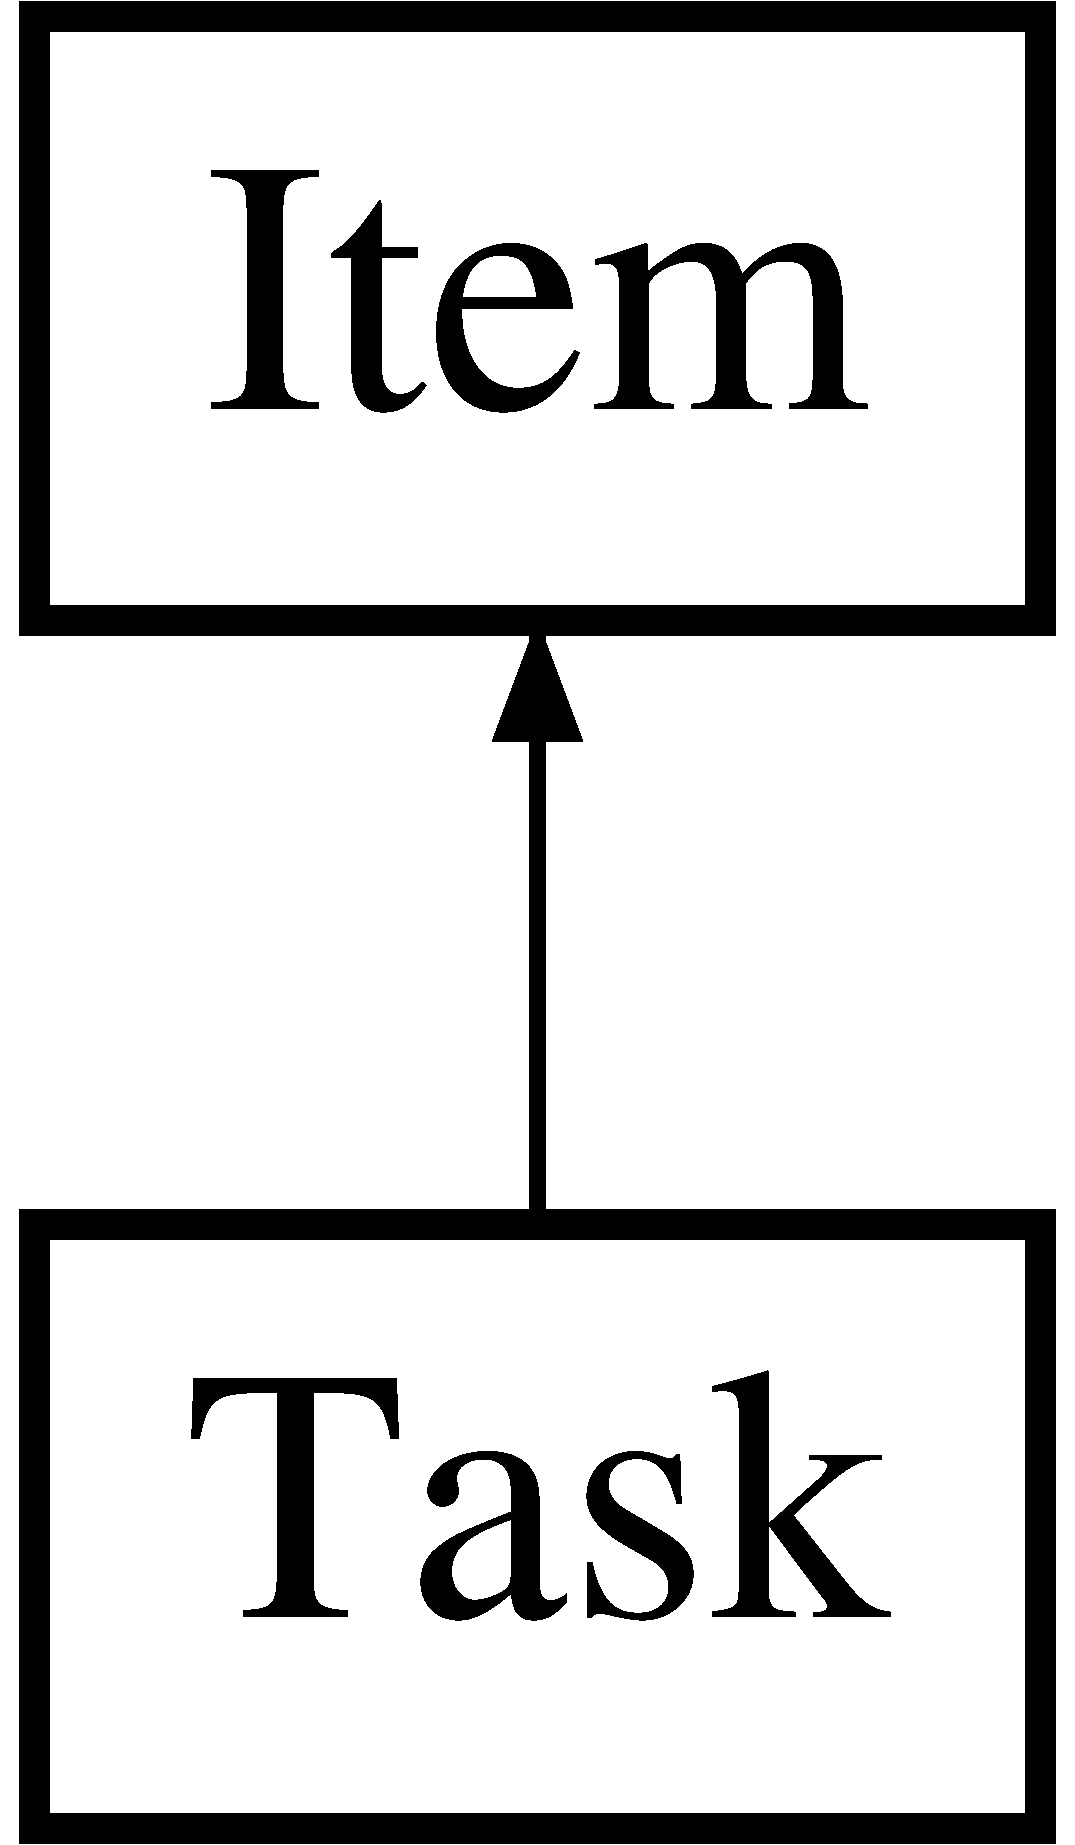
\includegraphics[height=2.000000cm]{class_task}
\end{center}
\end{figure}
\subsection*{Public Member Functions}
\begin{DoxyCompactItemize}
\item 
\mbox{\hyperlink{class_task_a43834b15cba574ccd4f25af665649776}{Task}} (std\+::string \&)
\item 
\mbox{\hyperlink{class_task_a60073fae7e07b8d1721b1bc73adcc6c8}{Task}} (\mbox{\hyperlink{class_task}{Task}} \&)=delete
\item 
\mbox{\hyperlink{class_task}{Task}} \& \mbox{\hyperlink{class_task_a95c7171fb2f939f1e4ae9a82f1c7c32d}{operator=}} (\mbox{\hyperlink{class_task}{Task}} \&)=delete
\item 
\mbox{\hyperlink{class_task_ae146c98551f244f62b93bc7b4e334580}{Task}} (\mbox{\hyperlink{class_task}{Task}} \&\&)=delete
\item 
\mbox{\hyperlink{class_task}{Task}} \& \mbox{\hyperlink{class_task_ada7e932e1a40e87069806c264ca3b2c5}{operator=}} (\mbox{\hyperlink{class_task}{Task}} \&\&)=delete
\item 
\mbox{\Hypertarget{class_task_a77d0a5c728a3d0bec89217afbd3addfd}\label{class_task_a77d0a5c728a3d0bec89217afbd3addfd}} 
void {\bfseries Run\+Process} (std\+::ostream \&os)
\item 
bool \mbox{\hyperlink{class_task_ad5f00535195117634b86714e628abd77}{Move\+Task}} ()
\item 
void \mbox{\hyperlink{class_task_aca65eac4162faecd7cce47db096183fc}{set\+Next\+Task}} (\mbox{\hyperlink{class_task}{Task}} \&task)
\item 
bool \mbox{\hyperlink{class_task_a6cfa898328059215d5a89f27aac7985b}{get\+Completed}} (\mbox{\hyperlink{class_customer_order}{Customer\+Order}} \&src)
\item 
void \mbox{\hyperlink{class_task_ad94a831f3fd8c66b41a1dd24f751cbb1}{Validate}} (std\+::ostream \&os)
\item 
\mbox{\hyperlink{class_task}{Task}} \& \mbox{\hyperlink{class_task_a3ed2681da2f886dc5742dc180f03a3b8}{operator+=}} (\mbox{\hyperlink{class_customer_order}{Customer\+Order}} \&\&new\+Order)
\end{DoxyCompactItemize}


\subsection{Constructor \& Destructor Documentation}
\mbox{\Hypertarget{class_task_a43834b15cba574ccd4f25af665649776}\label{class_task_a43834b15cba574ccd4f25af665649776}} 
\index{Task@{Task}!Task@{Task}}
\index{Task@{Task}!Task@{Task}}
\subsubsection{\texorpdfstring{Task()}{Task()}\hspace{0.1cm}{\footnotesize\ttfamily [1/3]}}
{\footnotesize\ttfamily Task\+::\+Task (\begin{DoxyParamCaption}\item[{std\+::string \&}]{abc }\end{DoxyParamCaption})}

Custom Constructor !$>$ \mbox{\Hypertarget{class_task_a60073fae7e07b8d1721b1bc73adcc6c8}\label{class_task_a60073fae7e07b8d1721b1bc73adcc6c8}} 
\index{Task@{Task}!Task@{Task}}
\index{Task@{Task}!Task@{Task}}
\subsubsection{\texorpdfstring{Task()}{Task()}\hspace{0.1cm}{\footnotesize\ttfamily [2/3]}}
{\footnotesize\ttfamily Task\+::\+Task (\begin{DoxyParamCaption}\item[{\mbox{\hyperlink{class_task}{Task}} \&}]{ }\end{DoxyParamCaption})\hspace{0.3cm}{\ttfamily [delete]}}

Uninitialized copy constructor !$>$ \mbox{\Hypertarget{class_task_ae146c98551f244f62b93bc7b4e334580}\label{class_task_ae146c98551f244f62b93bc7b4e334580}} 
\index{Task@{Task}!Task@{Task}}
\index{Task@{Task}!Task@{Task}}
\subsubsection{\texorpdfstring{Task()}{Task()}\hspace{0.1cm}{\footnotesize\ttfamily [3/3]}}
{\footnotesize\ttfamily Task\+::\+Task (\begin{DoxyParamCaption}\item[{\mbox{\hyperlink{class_task}{Task}} \&\&}]{ }\end{DoxyParamCaption})\hspace{0.3cm}{\ttfamily [delete]}}

Uninitialized move constructor !$>$ 

\subsection{Member Function Documentation}
\mbox{\Hypertarget{class_task_a6cfa898328059215d5a89f27aac7985b}\label{class_task_a6cfa898328059215d5a89f27aac7985b}} 
\index{Task@{Task}!get\+Completed@{get\+Completed}}
\index{get\+Completed@{get\+Completed}!Task@{Task}}
\subsubsection{\texorpdfstring{get\+Completed()}{getCompleted()}}
{\footnotesize\ttfamily bool Task\+::get\+Completed (\begin{DoxyParamCaption}\item[{\mbox{\hyperlink{class_customer_order}{Customer\+Order}} \&}]{src }\end{DoxyParamCaption})}

$<$ set the next available task for the order !$>$ complete the order on queue !$>$ \mbox{\Hypertarget{class_task_ad5f00535195117634b86714e628abd77}\label{class_task_ad5f00535195117634b86714e628abd77}} 
\index{Task@{Task}!Move\+Task@{Move\+Task}}
\index{Move\+Task@{Move\+Task}!Task@{Task}}
\subsubsection{\texorpdfstring{Move\+Task()}{MoveTask()}}
{\footnotesize\ttfamily bool Task\+::\+Move\+Task (\begin{DoxyParamCaption}{ }\end{DoxyParamCaption})}

$<$ fill last order on order queue !$>$ \mbox{\Hypertarget{class_task_a3ed2681da2f886dc5742dc180f03a3b8}\label{class_task_a3ed2681da2f886dc5742dc180f03a3b8}} 
\index{Task@{Task}!operator+=@{operator+=}}
\index{operator+=@{operator+=}!Task@{Task}}
\subsubsection{\texorpdfstring{operator+=()}{operator+=()}}
{\footnotesize\ttfamily \mbox{\hyperlink{class_task}{Task}} \& Task\+::operator+= (\begin{DoxyParamCaption}\item[{\mbox{\hyperlink{class_customer_order}{Customer\+Order}} \&\&}]{new\+Order }\end{DoxyParamCaption})}

move an order to the front of the queue !$>$ \mbox{\Hypertarget{class_task_a95c7171fb2f939f1e4ae9a82f1c7c32d}\label{class_task_a95c7171fb2f939f1e4ae9a82f1c7c32d}} 
\index{Task@{Task}!operator=@{operator=}}
\index{operator=@{operator=}!Task@{Task}}
\subsubsection{\texorpdfstring{operator=()}{operator=()}\hspace{0.1cm}{\footnotesize\ttfamily [1/2]}}
{\footnotesize\ttfamily \mbox{\hyperlink{class_task}{Task}}\& Task\+::operator= (\begin{DoxyParamCaption}\item[{\mbox{\hyperlink{class_task}{Task}} \&}]{ }\end{DoxyParamCaption})\hspace{0.3cm}{\ttfamily [delete]}}

Uninitialized copy assignment !$>$ \mbox{\Hypertarget{class_task_ada7e932e1a40e87069806c264ca3b2c5}\label{class_task_ada7e932e1a40e87069806c264ca3b2c5}} 
\index{Task@{Task}!operator=@{operator=}}
\index{operator=@{operator=}!Task@{Task}}
\subsubsection{\texorpdfstring{operator=()}{operator=()}\hspace{0.1cm}{\footnotesize\ttfamily [2/2]}}
{\footnotesize\ttfamily \mbox{\hyperlink{class_task}{Task}}\& Task\+::operator= (\begin{DoxyParamCaption}\item[{\mbox{\hyperlink{class_task}{Task}} \&\&}]{ }\end{DoxyParamCaption})\hspace{0.3cm}{\ttfamily [delete]}}

Uninitialized move assignment !$>$ \mbox{\Hypertarget{class_task_aca65eac4162faecd7cce47db096183fc}\label{class_task_aca65eac4162faecd7cce47db096183fc}} 
\index{Task@{Task}!set\+Next\+Task@{set\+Next\+Task}}
\index{set\+Next\+Task@{set\+Next\+Task}!Task@{Task}}
\subsubsection{\texorpdfstring{set\+Next\+Task()}{setNextTask()}}
{\footnotesize\ttfamily void Task\+::set\+Next\+Task (\begin{DoxyParamCaption}\item[{\mbox{\hyperlink{class_task}{Task}} \&}]{task }\end{DoxyParamCaption})}

$<$ move move completed task to next part !$>$ \mbox{\Hypertarget{class_task_ad94a831f3fd8c66b41a1dd24f751cbb1}\label{class_task_ad94a831f3fd8c66b41a1dd24f751cbb1}} 
\index{Task@{Task}!Validate@{Validate}}
\index{Validate@{Validate}!Task@{Task}}
\subsubsection{\texorpdfstring{Validate()}{Validate()}}
{\footnotesize\ttfamily void Task\+::\+Validate (\begin{DoxyParamCaption}\item[{std\+::ostream \&}]{os }\end{DoxyParamCaption})}

validate the next available task !$>$ 

The documentation for this class was generated from the following files\+:\begin{DoxyCompactItemize}
\item 
Task.\+h\item 
Task.\+cpp\end{DoxyCompactItemize}

\hypertarget{class_utilities}{}\section{Utilities Class Reference}
\label{class_utilities}\index{Utilities@{Utilities}}
\subsection*{Public Member Functions}
\begin{DoxyCompactItemize}
\item 
\mbox{\hyperlink{class_utilities_ab1676c9ce35cf347a73d16f1094e1271}{Utilities}} ()
\item 
void \mbox{\hyperlink{class_utilities_ac988cf9fa28095c6e5e478364a7115af}{set\+Field\+Width}} (size\+\_\+t)
\item 
size\+\_\+t \mbox{\hyperlink{class_utilities_a4d76700f1ca78a0fcac71661ac05a137}{get\+Field\+Width}} () const
\item 
const std\+::string \mbox{\hyperlink{class_utilities_a965e959066042decc812c4e8b8602a7e}{extract\+Token}} (const std\+::string \&, size\+\_\+t \&, bool \&)
\item 
const char \mbox{\hyperlink{class_utilities_a8335fa01c68450eceb6f409fd6c2469d}{get\+Delimiter}} () const
\end{DoxyCompactItemize}
\subsection*{Static Public Member Functions}
\begin{DoxyCompactItemize}
\item 
static void \mbox{\hyperlink{class_utilities_a6961ff17f2a37332cff6ef51940b9c7b}{set\+Delimiter}} (const char)
\end{DoxyCompactItemize}


\subsection{Constructor \& Destructor Documentation}
\mbox{\Hypertarget{class_utilities_ab1676c9ce35cf347a73d16f1094e1271}\label{class_utilities_ab1676c9ce35cf347a73d16f1094e1271}} 
\index{Utilities@{Utilities}!Utilities@{Utilities}}
\index{Utilities@{Utilities}!Utilities@{Utilities}}
\subsubsection{\texorpdfstring{Utilities()}{Utilities()}}
{\footnotesize\ttfamily Utilities\+::\+Utilities (\begin{DoxyParamCaption}{ }\end{DoxyParamCaption})}

Default Constructor !$>$ 

\subsection{Member Function Documentation}
\mbox{\Hypertarget{class_utilities_a965e959066042decc812c4e8b8602a7e}\label{class_utilities_a965e959066042decc812c4e8b8602a7e}} 
\index{Utilities@{Utilities}!extract\+Token@{extract\+Token}}
\index{extract\+Token@{extract\+Token}!Utilities@{Utilities}}
\subsubsection{\texorpdfstring{extract\+Token()}{extractToken()}}
{\footnotesize\ttfamily const string Utilities\+::extract\+Token (\begin{DoxyParamCaption}\item[{const std\+::string \&}]{,  }\item[{size\+\_\+t \&}]{,  }\item[{bool \&}]{ }\end{DoxyParamCaption})}

function break down string, begin a certain position and stop at deliminator !$>$ \mbox{\Hypertarget{class_utilities_a8335fa01c68450eceb6f409fd6c2469d}\label{class_utilities_a8335fa01c68450eceb6f409fd6c2469d}} 
\index{Utilities@{Utilities}!get\+Delimiter@{get\+Delimiter}}
\index{get\+Delimiter@{get\+Delimiter}!Utilities@{Utilities}}
\subsubsection{\texorpdfstring{get\+Delimiter()}{getDelimiter()}}
{\footnotesize\ttfamily const char Utilities\+::get\+Delimiter (\begin{DoxyParamCaption}{ }\end{DoxyParamCaption}) const}

function return delimiter !$>$ \mbox{\Hypertarget{class_utilities_a4d76700f1ca78a0fcac71661ac05a137}\label{class_utilities_a4d76700f1ca78a0fcac71661ac05a137}} 
\index{Utilities@{Utilities}!get\+Field\+Width@{get\+Field\+Width}}
\index{get\+Field\+Width@{get\+Field\+Width}!Utilities@{Utilities}}
\subsubsection{\texorpdfstring{get\+Field\+Width()}{getFieldWidth()}}
{\footnotesize\ttfamily std\+::size\+\_\+t Utilities\+::get\+Field\+Width (\begin{DoxyParamCaption}{ }\end{DoxyParamCaption}) const}

function return field\+\_\+width length !$>$ \mbox{\Hypertarget{class_utilities_a6961ff17f2a37332cff6ef51940b9c7b}\label{class_utilities_a6961ff17f2a37332cff6ef51940b9c7b}} 
\index{Utilities@{Utilities}!set\+Delimiter@{set\+Delimiter}}
\index{set\+Delimiter@{set\+Delimiter}!Utilities@{Utilities}}
\subsubsection{\texorpdfstring{set\+Delimiter()}{setDelimiter()}}
{\footnotesize\ttfamily void Utilities\+::set\+Delimiter (\begin{DoxyParamCaption}\item[{const char}]{delim }\end{DoxyParamCaption})\hspace{0.3cm}{\ttfamily [static]}}

set delimiter to break down string !$>$ \mbox{\Hypertarget{class_utilities_ac988cf9fa28095c6e5e478364a7115af}\label{class_utilities_ac988cf9fa28095c6e5e478364a7115af}} 
\index{Utilities@{Utilities}!set\+Field\+Width@{set\+Field\+Width}}
\index{set\+Field\+Width@{set\+Field\+Width}!Utilities@{Utilities}}
\subsubsection{\texorpdfstring{set\+Field\+Width()}{setFieldWidth()}}
{\footnotesize\ttfamily void Utilities\+::set\+Field\+Width (\begin{DoxyParamCaption}\item[{size\+\_\+t}]{ }\end{DoxyParamCaption})}

set field\+\_\+width with a value !$>$ 

The documentation for this class was generated from the following files\+:\begin{DoxyCompactItemize}
\item 
Utilities.\+h\item 
Assembly\+Line.\+cpp\item 
Utilities.\+cpp\end{DoxyCompactItemize}

%--- End generated contents ---

% Index
\backmatter
\newpage
\phantomsection
\clearemptydoublepage
\addcontentsline{toc}{chapter}{Index}
\printindex

\end{document}
